\documentclass[11pt,a4j]{jsarticle}
\usepackage{float,array,booktabs,here}
\usepackage{amsmath}
\usepackage{bm}
\usepackage[dvipdfmx]{graphicx}
\usepackage{listings}
%\usepackage[whole]{bxcjkjatype}%日本語もコンパイル可にする.
%\usepackage[dvipdfmx,hiresbb]{graphicx}
\usepackage[top=25truemm,bottom=25truemm,left=25truemm,right=25truemm]{geometry}

\title{画像処理プログラミング}
\author{61401007 情報工学科 3年 飯塚 健介}
\date{\today}
\begin{document}
    \maketitle
    \section{開発環境について}
    今回の画像処理を実装するにあたり、以下の開発環境を利用した。
    \begin{itemize}
        \item Python3.5.2
        \item NumPy (Pythonの数値計算ライブラリ)
        \item OpenCV(画像の読み込みと書き出しのみに使用)
    \end{itemize}
    レポートにソースコードを挿入する関係で一部、実際のプログラムとは異なるインデントとなってしまっている。
    \section{実装した処理の一覧}
    課題から以下の一覧の処理を実装した。それぞれ利用したアルゴリズム、実装したソースコード、処理結果とその検討を記す。
    \begin{itemize}
        \item 空間フィルタリング(平滑化、微分、鮮鋭化)
        \item ノイズ除去(メディアンフィルタ、バイラテラルフィルタ)
        \item ハーフトーン処理(ディザ法、誤差拡散法)
        \item ガンマ変換
        \item ヒストグラム平坦化
        \item 射影変換
        \item HDR合成
    \end{itemize}
    \section{空間フィルタリング}
    平滑化フィルタ、微分フィルタ、鮮鋭化フィルタを実装した。
    平滑化は濃淡変化を滑らかにすることで画像に含まれるノイズなどの不要な濃淡変動を軽減するために用いられる。微分フィルタは画像のエッジ抽出を行うために用いられる。
    鮮鋭化フィルタは微分フィルタがエッジのみを残すのに対して、入力画像の濃淡を残したまま、エッジを強調するフィルタである。
    \subsection{実装したコード}
    image\_filtering関数ではフィルタと画素の行列計算をsmoothed\_filteringで平滑化、diff\_filteringで横方向微分、sharpened\_filteringで鮮鋭化、edge\_detection\_filteringでエッジ抽出(Sobelフィルタを使用)を実装している。

    \begin{lstlisting}[basicstyle=\ttfamily\footnotesize, frame=single]
      def image_filtering(filter_matrix, input_img, output_img):
        img_height = input_img.shape[0]
        img_width = input_img.shape[1]
        for i in range(1, img_height - 1):
          for j in range(1, img_width - 1):
            for k in range(-1, 2):
              for l in range(-1, 2):
                output_img[i][j] += filter_matrix[k + 1][l + 1] *
                                    input_img[i + k][j + l]
          int(output_img[i][j])

      def smoothed_filtering(input_img, output_img):
        smoothed_filter = np.array([[1, 1, 1], [1, 1, 1], [1, 1, 1]]) / 9
        image_filtering(smoothed_filter, input_img, output_img)


      def sharpened_filtering(input_img, output_img):
        sharpened_filter = np.array([[-1, -1, -1], [-1, 9, -1], [-1, -1, -1]])
        image_filtering(sharpened_filter, input_img, output_img)

      def diff_filtering(input_img, output_img):
          diff_filter = np.array([[0, 0, 0], [-1, 1, 0], [0, 0, 0]])
          image_filtering(diff_filter, input_img, output_img)


      def edge_detection_filtering(input_img, output_img):
          img_height = input_img.shape[0]
          img_width = input_img.shape[1]
          yoko_result = np.zeros((img_height, img_width))
          tate_result = np.zeros((img_height, img_width))
          edge_yoko_filter = np.array([[-1, 0, 1], [-2, 0, 2], [-1, 0, 1]])
          edge_tate_filter = np.array([[-1, -2, -1], [0, 0, 0], [1, 2, 1]])
          image_filtering(edge_yoko_filter, input_img, yoko_result)
          image_filtering(edge_tate_filter, input_img, tate_result)
          for i in range(img_height):
              for j in range(img_width):
                  tmp = np.sqrt(yoko_result[i][j] ** 2 + tate_result[i][j] ** 2)
                  if tmp > 255:
                      output_img[i][j] = 255
                  elif tmp < 0:
                      output_img[i][j] = 0
                  else:
                      output_img[i][j] = tmp

    \end{lstlisting}

    \subsection{処理結果}
    \begin{figure}[H]
      \centering
      \includegraphics[clip,width=16.0cm ,height= 9.0cm]{./img/smoothed/smoothed_source.png}
      \caption{平滑化入力画像\label{fig:smoothed_source}}
    \end{figure}
    \begin{figure}[H]
      \centering
      \includegraphics[clip,width=16.0cm ,height= 9.0cm]{./img/smoothed/smoothed.png}
      \caption{平滑化出力画像\label{fig:smoothed_result}}
    \end{figure}

    \begin{figure}[H]
      \centering
      \includegraphics[clip,width=12.0cm ,height= 9.6cm]{./img/sharpened/sharpened_source.png}
      \caption{鮮鋭化入力画像(http://www.bing.com/gallery/\#images/AthabascaCanyon)\label{fig:sharpened_source}}
    \end{figure}
    \begin{figure}[H]
      \centering
      \includegraphics[clip,width=12.0cm ,height= 9.6cm]{./img/sharpened/sharpened.png}
      \caption{鮮鋭化出力画像\label{fig:sharpened_result}}
    \end{figure}

    \begin{figure}[H]
      \centering
      \includegraphics[clip,width=10.0cm ,height= 7.5cm]{./img/diff_edge/diff_edge_source.png}
      \caption{微分,エッジ抽出入力画像\label{fig:diff_source}}
    \end{figure}
    \begin{figure}[H]
      \centering
      \includegraphics[clip,width=10.0cm ,height= 7.5cm]{./img/diff_edge/diff.png}
      \caption{微分出力画像\label{fig:diff_result}}
    \end{figure}

    \begin{figure}[H]
      \centering
      \includegraphics[clip,width=10.0cm ,height= 7.5cm]{./img/diff_edge/edge.png}
      \caption{エッジ抽出出力画像\label{fig:edge_detect_result}}
    \end{figure}
    \subsection{検討}
    平滑化については、画像がぼやけたように変化するので輪郭がしっかりしている文字が含まれた画像を選び、出力画像の文字が入力画像の文字に比べてぼやけて見えることで結果を確認しやすいようにした。
    結果をみるときちんと処理がなされていることが確認できる。
    鮮鋭化は、エッジとなる線がよりはっきり表れるのでbingの壁紙となっていた雪山の崖を選んだ。これにより雪の積層や崖の地層の間の線などが明瞭になっていることが確認できた。
    微分、エッジ抽出については窓や輪郭が直線で分かりやすい建物の写真を用いた。微分は横方向微分を実行したので、窓枠などの縦線のみが残り、エッジ抽出はSobelフィルタを用いて建物の窓枠や輪郭が抽出されていることがわかる。
    全てのフィルタで目的の画像を得られた。
    \section{ノイズ除去}
    メディアンフィルタ、バイラテラルフィルタを実装した。また前節の平滑化フィルタも含めて比較検討する。
    これらはノイズ除去を目的としたフィルタであるがメディアンフィルタはスパイク状のノイズを除去するのに適している。バイラテラルフィルタは平滑化フィルタに比べて、エッジを保存したまま、ノイズを除去する事ができる。
    \subsection{実装したコード}
    median\_filteringでメディアンフィルタを、bilateral\_filteringでバイラテラルフィルタを実装した。またmedian関数で各画素に代入する中央値を算出している。
    \begin{lstlisting}[basicstyle=\ttfamily\footnotesize, frame=single]
        def median_filtering(n, m, input_img, output_img):
            img_height = input_img.shape[0]
            img_width = input_img.shape[1]

            for i in range(1, img_height - 1):
                for j in range(1, img_width - 1):
                    output_img[i][j] = median(n, m, input_img, i, j)


        def median(n, m, input_img, i, j):
            median_value = 0
            count = 0
            median_list = np.zeros(n * m)
            for k in range(-1, 2):
                for l in range(-1, 2):
                    median_list[count] = input_img[i + k][ j + l]
                    count += 1
            median_value = np.median(median_list)
            return int(median_value)


        def bilateral_filtering(input_img, output_img, s1, s2, W):
            img_height = input_img.shape[0]
            img_width = input_img.shape[1]
            work = np.zeros((img_height, img_width))
            for i in range(W, img_height - W):
                for j in range(W, img_width - W):
                    weighten_pix = 0
                    sum_weight = 0
                    weight = 0
                    float(weight)
                    for k in range(-W, W + 1):
                        for l in range(-W, W + 1):
                            im1 = input_img[i][j]
                            im2 = input_img[i + k][j + l]
                            w2_tmp = im1 - im2
                            w2_tmp = (w2_tmp) * (w2_tmp) / -(2 * s2 ** 2)
                            weight = np.exp(-(k ** 2 + l ** 2) / (2 * s1 ** 2)) *
                                     np.exp(w2_tmp)
                            sum_weight += weight
                            weighten_pix += im2 * weight
                    work[i][j] = weighten_pix / sum_weight
                    print(work[i][j])
                    output_img[i][j] = int(work[i][j])
    \end{lstlisting}
    \subsection{処理結果}
    \begin{figure}[H]
      \centering
      \includegraphics[clip,width=13.0cm ,height= 3.5cm]{./img/median/median_source.png}
      \caption{メディアンフィルタ入力画像(http://www.airnewzealand.jp/newzealand-starwatching)\label{fig:median_source}}
    \end{figure}
    \begin{figure}[H]
      \centering
      \includegraphics[clip,width=13.0cm ,height= 3.5cm]{./img/median/median.png}
      \caption{メディアンフィルタ出力画像\label{fig:median_result}}
    \end{figure}

    \begin{figure}[H]
      \centering
      \includegraphics[clip,width=13.0cm ,height= 3.5cm]{./img/median/smoothedconv.png}
      \caption{平滑化フィルタ出力画像\label{fig:median_result}}
    \end{figure}

    \begin{figure}[H]
      \centering
      \includegraphics[clip,width=7.0cm ,height= 7.0cm]{./img/bilateral/bi_source.png}
      \caption{バイラテラルフィルタ入力画像(http://imagingsolution.net/imaging/bilateralfilter/)\label{fig:bilateral_source}}
    \end{figure}
    \begin{figure}[H]
      \centering
      \includegraphics[clip,width=7.0cm ,height= 7.0cm]{./img/bilateral/bi.png}
      \caption{バイラテラルフィルタ出力画像\label{fig:bilateral_result}}
    \end{figure}

    \subsection{検討}
    3×3のブロックでメディアンフィルタ処理を行った。
    メディアンフィルタについては星空の写真の星をスパイク状のノイズと見立てて処理したところ、星空から星が減っていることからスパイク状のノイズ除去ができたと考えられる。
    また同じ画像を平滑化したときと比べてエッジが保存されていることが家の壁や、下の英語の文字を比較して見るとわかる。
    バイラテラルフィルタは授業の理論式を元にプログラムを組んでみたが、計算のオーバーフローのエラーが出てしまい、プログラムが上手く動かなかった。
    出力結果を見ると、全体がぼけてしまい、理論式のガウシアンに近い処理だけが中途半端に実行されてしまったと考えられる。
    \section{ハーフトーン処理}
    ハーフトーン処理は,グレースケールの画像を白と黒のみの2値画像とするために用いられる。ディザ法と誤差拡散法の2つの方法で実装した。
    \subsection{実装したコード}
    \begin{lstlisting}[basicstyle=\ttfamily\footnotesize, frame=single]
        def dither_halftone(input_img, output_img):
            img_height = input_img.shape[0]
            img_width = input_img.shape[1]
            dmatrix = np.array([[0, 8, 2, 10],[12, 4, 14, 6],
                   [3, 11, 1, 9], [15, 7, 13, 5]])
            block_height = img_height // 4
            block_width = img_width // 4
            for i in range(0, block_height):
                for j in range(0, block_width):
                    for k in range(0, 4):
                        for l in range(0, 4):
                            yp = i * 4 + k
                            xp = j * 4 + l
                            if input_img[xp][yp] <= (dmatrix[k][l] * 16 + 8):
                                output_img[xp][yp] = 0
                            else:
                                output_img[xp][yp] = 255



        def error_diffusion_halftone(input_img, output_img):
            img_height = input_img.shape[0]
            img_width = input_img.shape[1]
            work = np.zeros((img_height, img_width), np.uint8)
            for i in range(0, img_height):
                for j in range(0, img_width -0):
                    work[i][j] = input_img[i][j]

            for i in range(1, img_height - 1):
                for j in range(1, img_width - 1):
                    if work[i][j] <= 127:
                        error = work[i][j] - 0
                        work[i][j] = 0
                    else:
                        error = work[i][j] - 255
                        work[i][j] = 255
                    work[i + 1][j] += (5 / 16) * error
                    work[i + 1][j + 1] += (3 / 16) * error
                    work[i][j + 1] += (5 / 16) * error
                    work[i - 1][j + 1] += (3 / 16) * error

            for i in range(img_height):
                for j in range(img_width):
                    output_img[i][j] = 255

            for i in range(0, img_height - 1):
                for j in range(1, img_width - 1):
                    if work[i][j] > 255:
                        output_img[i][j] = 255
                    elif work[i][j] < 0:
                        output_img[i][j] = 0
                    else:
                        output_img[i][j] = int(work[i][j])
    \end{lstlisting}
    \subsection{処理結果}
    \begin{figure}[H]
      \centering
      \includegraphics[clip,width=7.0cm ,height= 7.0cm]{./img/halftone/halftone_source.png}
      \caption{ハーフトーン入力画像(https://www.cosy.sbg.ac.at/~pmeerw/Watermarking/lena.html)\label{fig:halftone_source}}
    \end{figure}
    \begin{figure}[H]
      \centering
      \includegraphics[clip,width=7.0cm ,height= 7.0cm]{./img/halftone/dither.png}
      \caption{ディザ法出力画像\label{fig:dither_result}}
    \end{figure}
    \begin{figure}[H]
      \centering
      \includegraphics[clip,width=7.0cm ,height= 7.0cm]{./img/halftone/error.png}
      \caption{誤差拡散法出力画像\label{fig:error_result}}
    \end{figure}
    \subsection{検討}
    目的の画像が得られた。
    人物像の肌のきめ細かさなどをハーフトーン処理においてディザ法と誤差拡散法で比較したかったので,画像処理では有名なlenaの画像を入力画像とした。
    実際に両者の出力画像を比較すると、誤差拡散法のほうが、よりきめ細かい肌を表現していて、lenaの陰影や背景の陰影の具合もより入力画像に近くなっている。

    \section{ガンマ変換}
    ガンマ変換は画素の濃淡を変化させることによって画像の明るさを調整できる。
    また折れ線のトーンカーブでは水平部分で画素値が一定となってしまい、入力画像のその範囲の濃淡変化が失われてしまうが、ガンマ変換によろ曲線トーンカーブではその範囲を補うことができる。
    \subsection{実装したコード}
    \begin{lstlisting}[basicstyle=\ttfamily\footnotesize, frame=single]
        def gamma_translation(gamma, input_img, output_img):
            img_height = input_img.shape[0]
            img_width = input_img.shape[1]
            for i in range(img_height):
                for j in range(img_width):
                    tmp_pixel = 255 * (input_img[i][j] / 255) ** (1 / gamma)
                    output_img.itemset((i, j), int(tmp_pixel))
    \end{lstlisting}
    \subsection{処理結果}
    \begin{figure}[H]
      \centering
      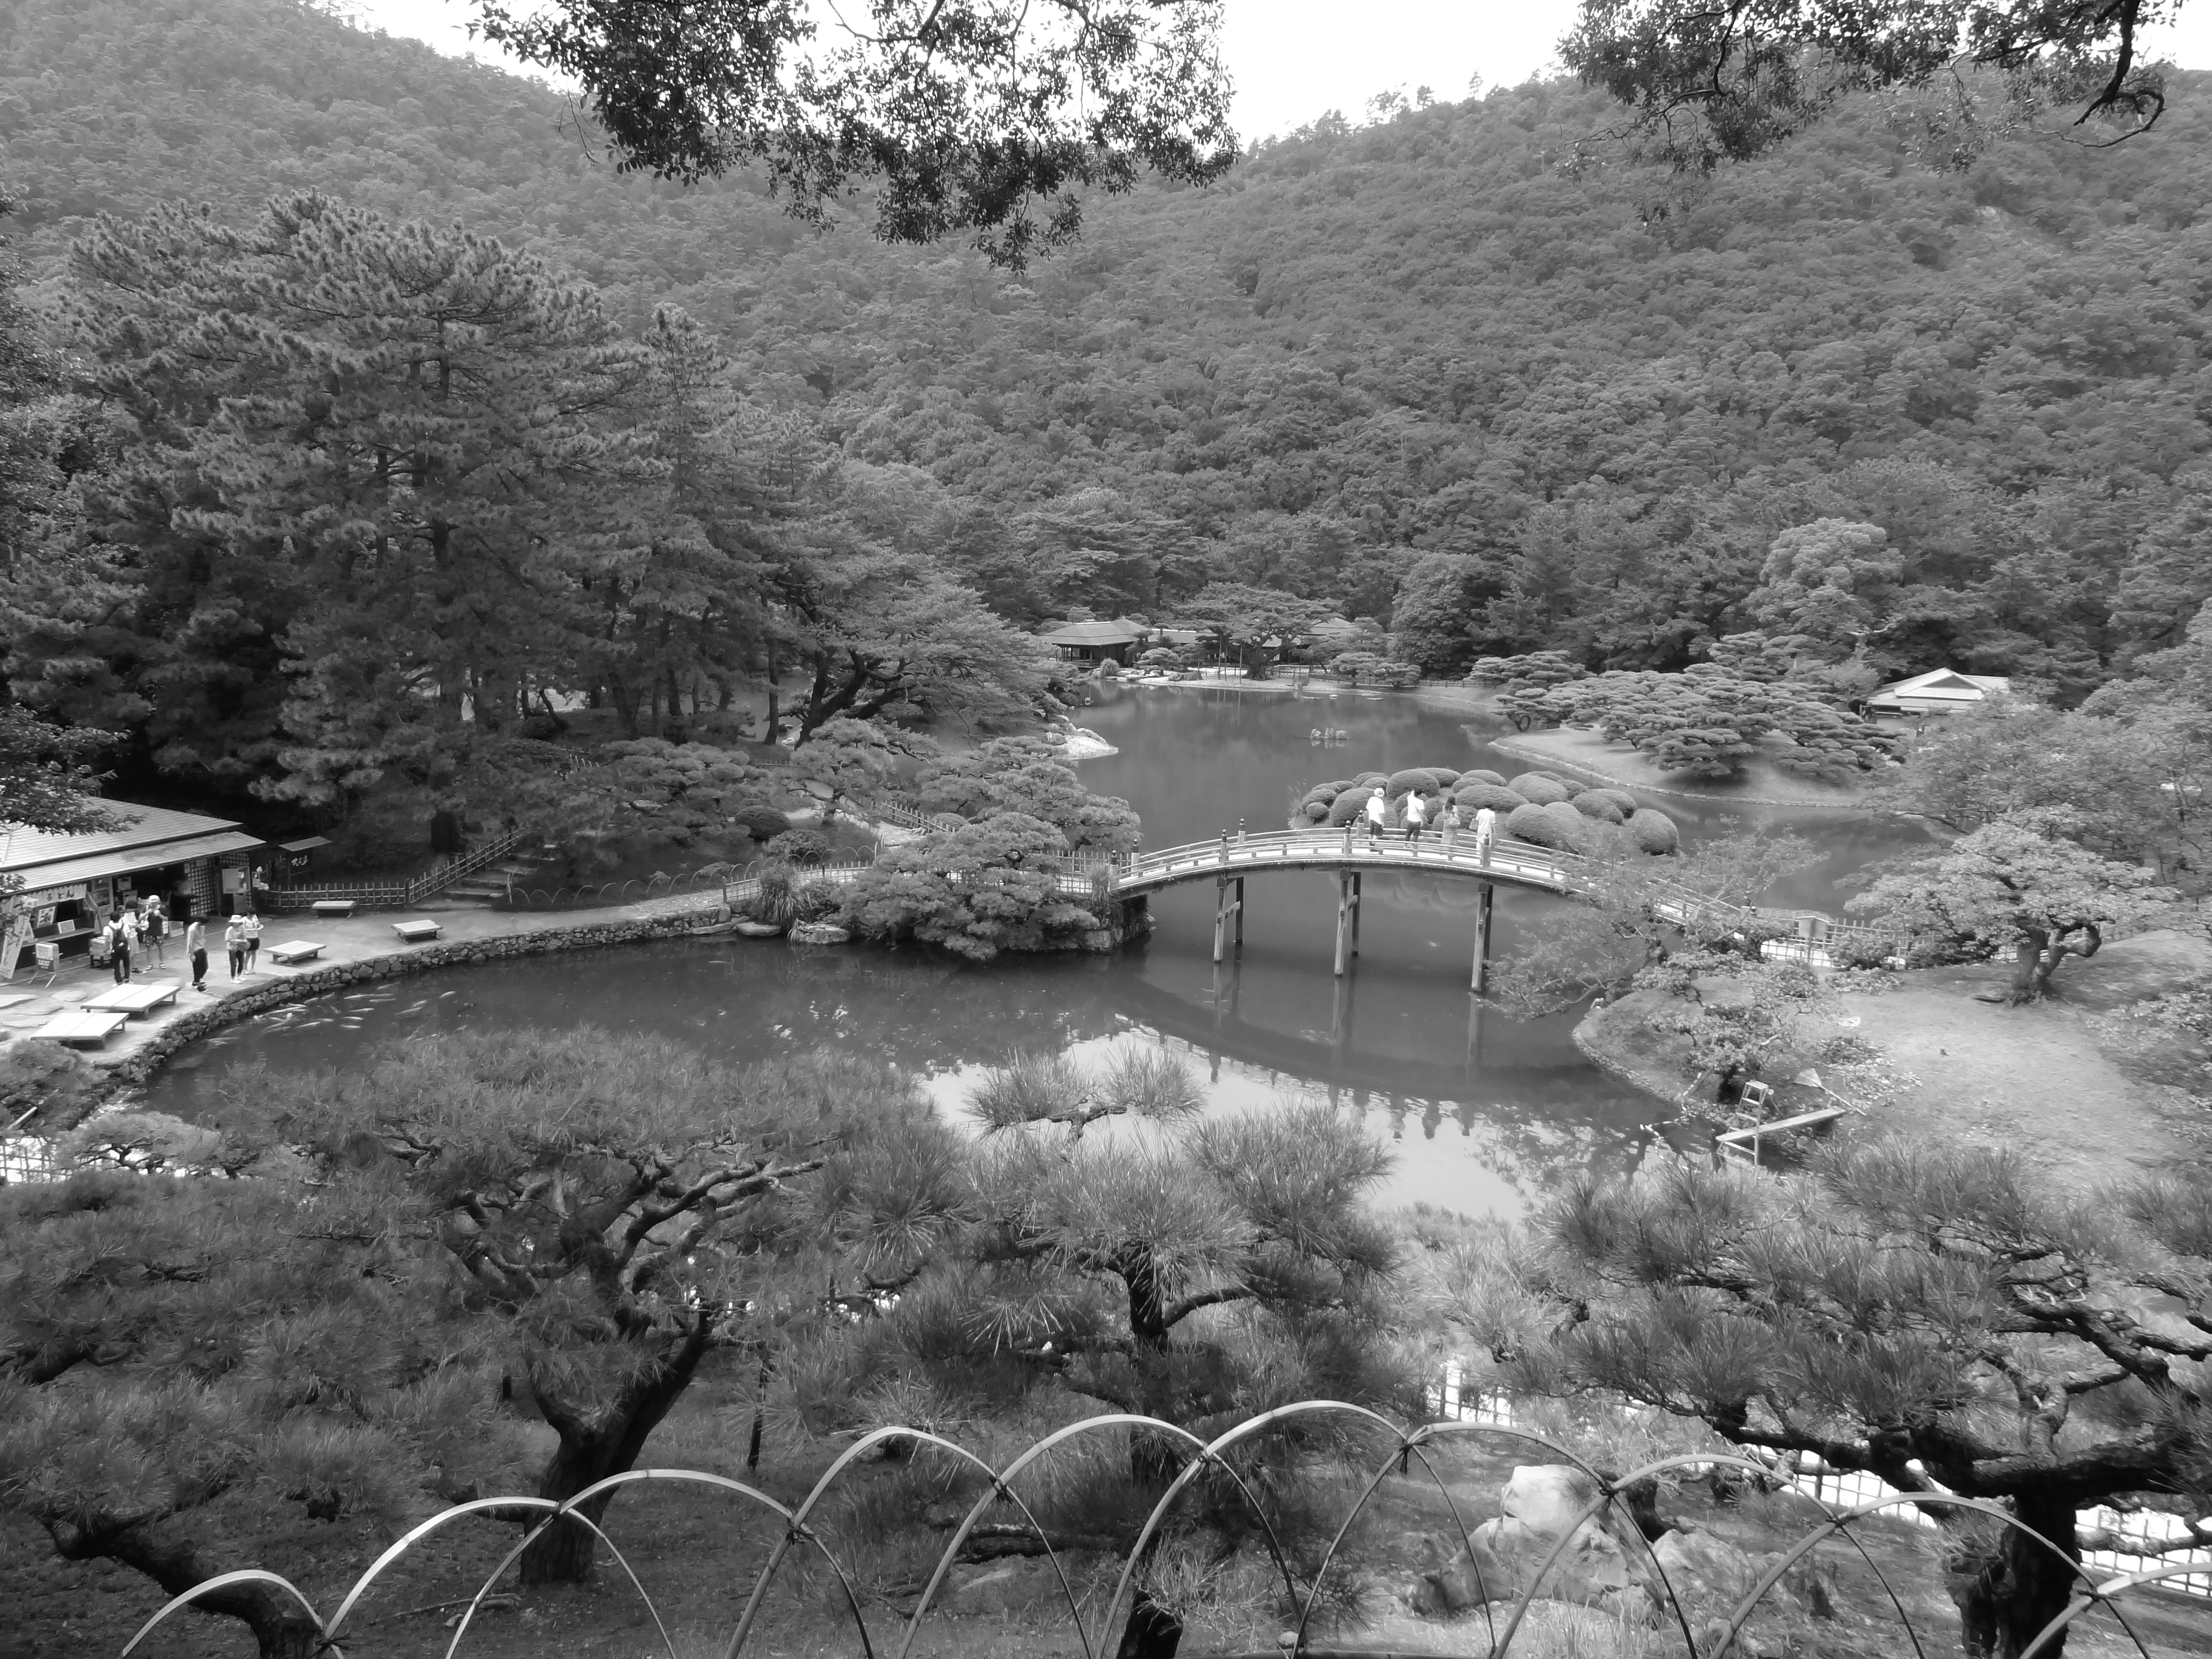
\includegraphics[clip,width=14cm ,height= 10cm]{./img/gamma/gamma_source.png}
      \caption{ガンマ変換入力画像\label{fig:gamma_source}}
    \end{figure}
    \begin{figure}[H]
      \centering
      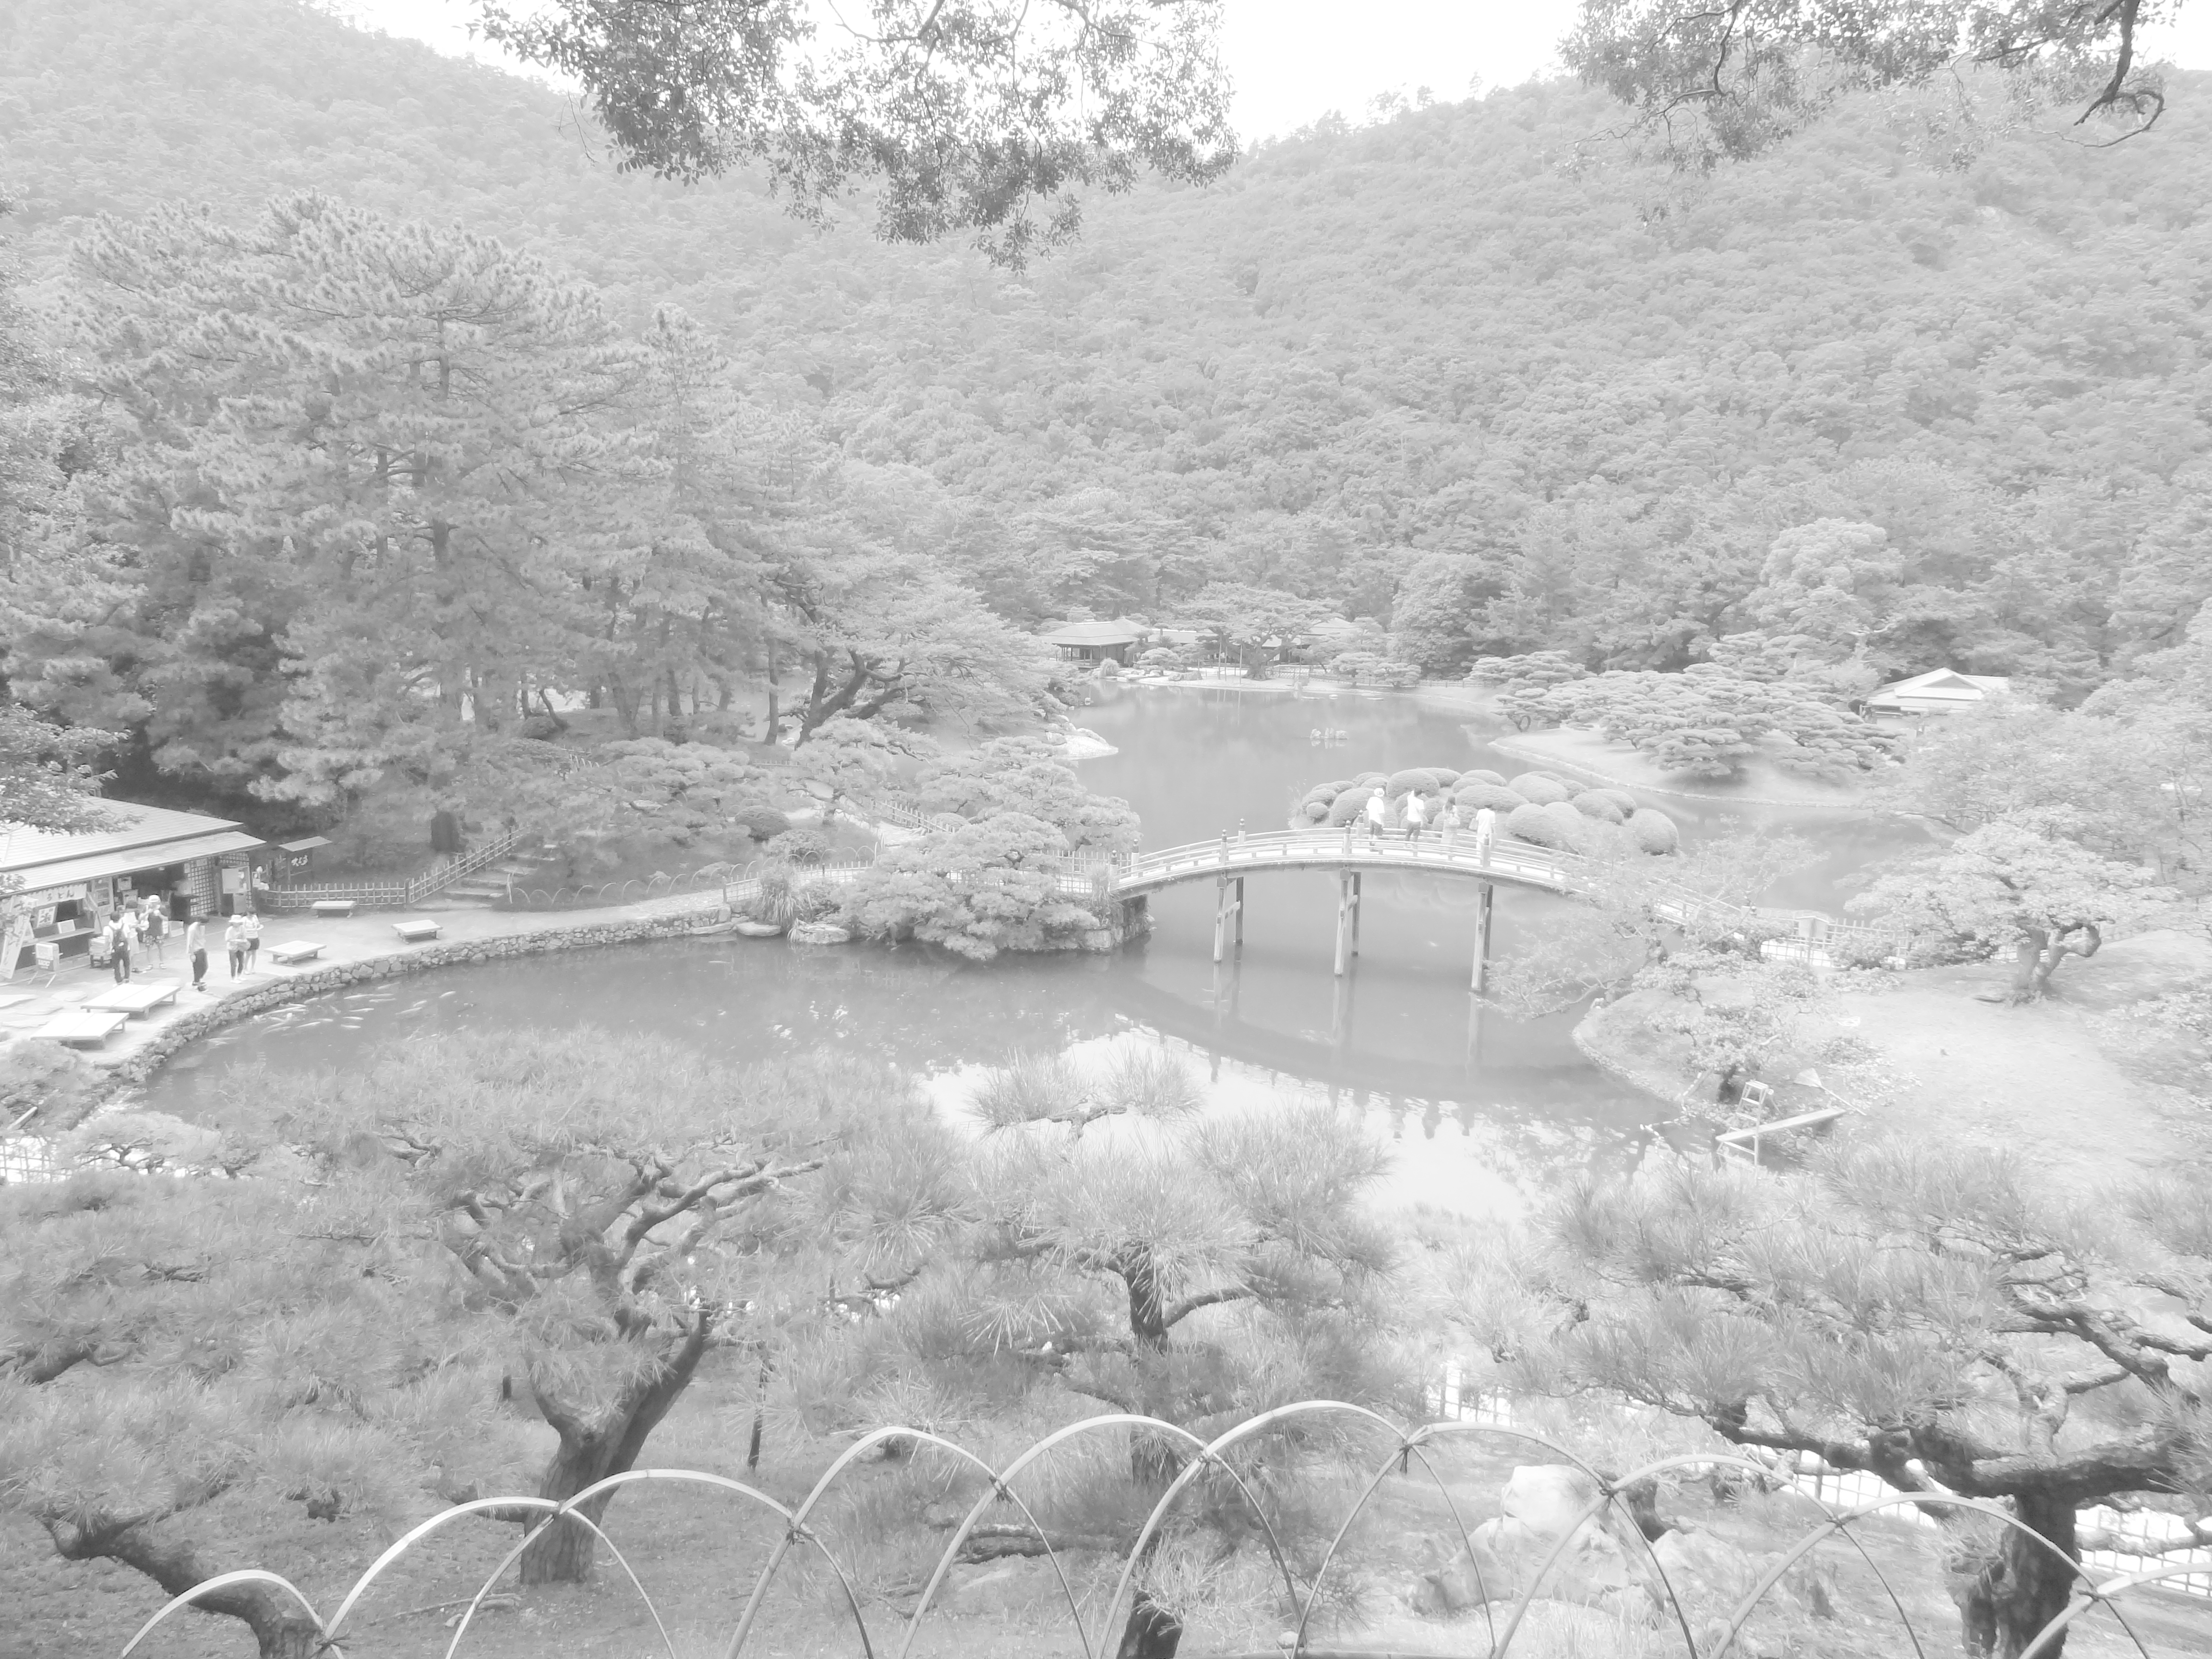
\includegraphics[clip,width=14cm ,height= 10cm]{./img/gamma/gamma3.png}
      \caption{$\gamma = 3$のときの出力画像\label{fig:gamma_result}}
    \end{figure}
    \begin{figure}[H]
      \centering
      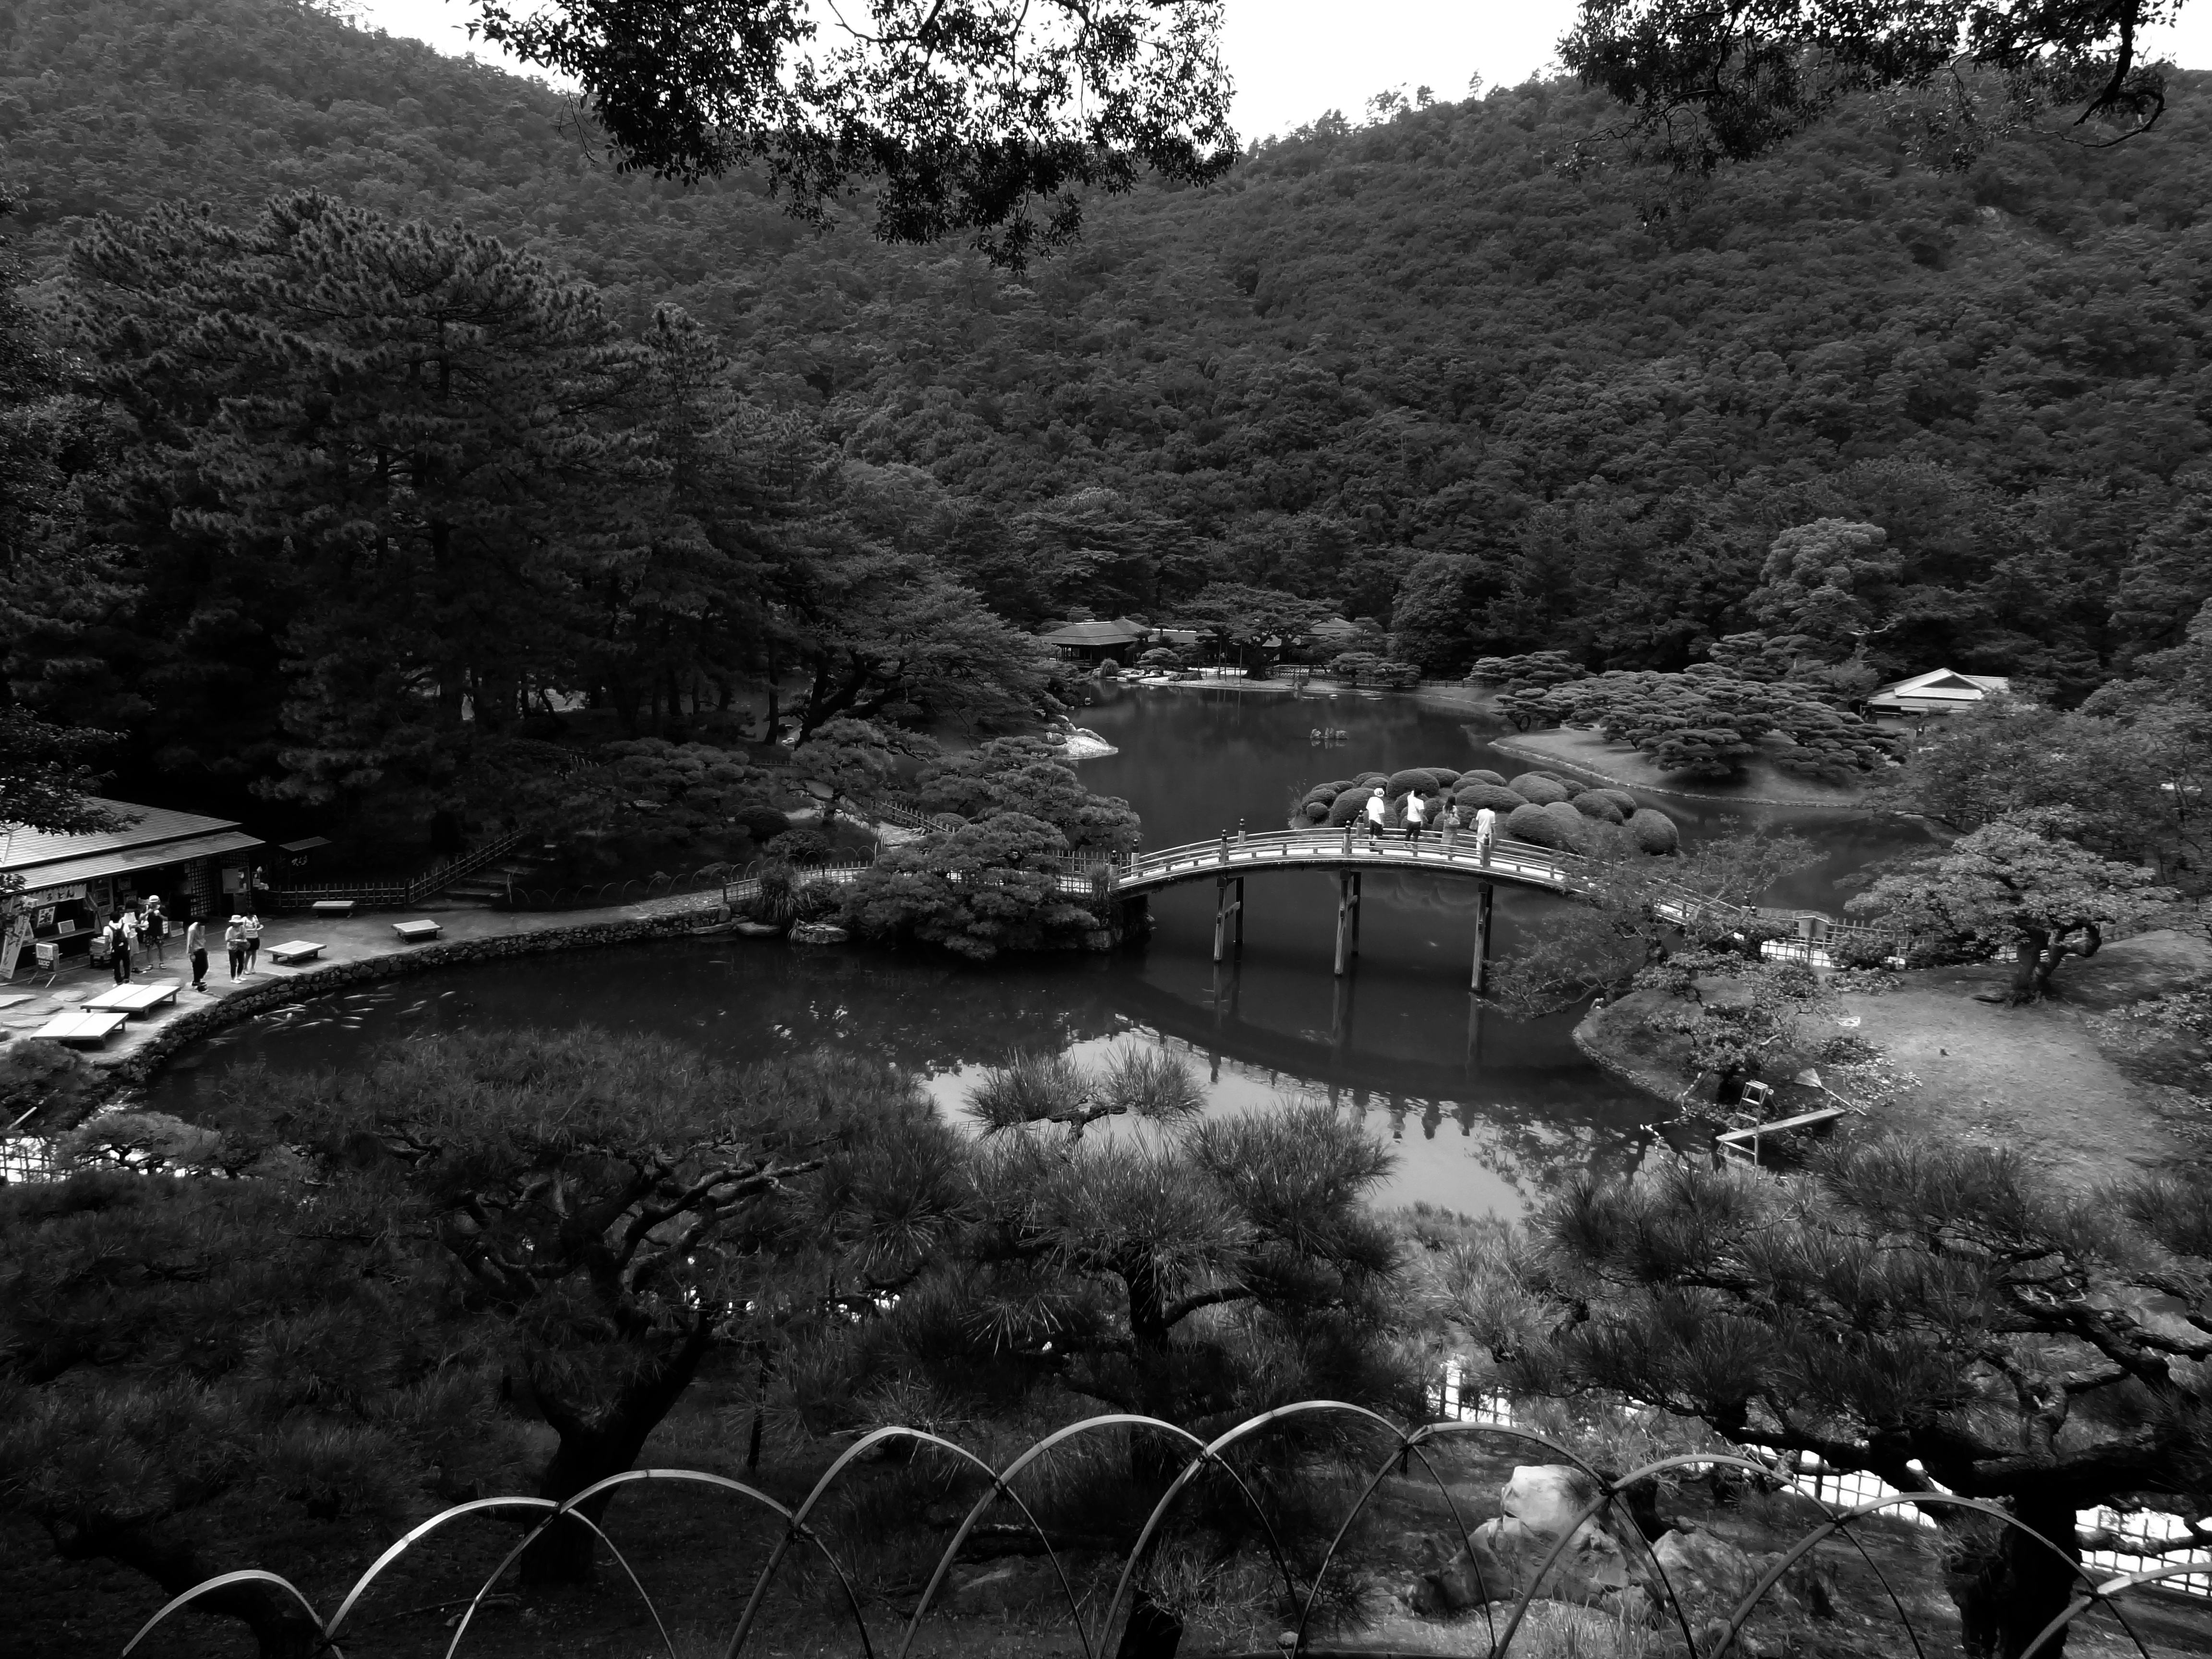
\includegraphics[clip,width=14cm ,height= 10cm]{./img/gamma/gamma05.png}
      \caption{$\gamma = 0.5$のときの出力画像\label{fig:gammas_result}}
    \end{figure}
    \subsection{検討}
    目的の画像が得られた。
    同じ画像についてそれぞれ$\gamma$の値をそれぞれ、$3$,$0.5$として処理した。入力画像に比べて$\gamma = 3$は明るくなり、$\gamma = 0.5$のときは暗くなった。
    \section{ヒストグラム平坦化}
    濃淡変化を行い、画像のコントラストを上げるためにヒストグラム平坦化は用いられる。
    \subsection{実装したコード}
    \begin{lstlisting}[basicstyle=\ttfamily\footnotesize, frame=single]
        def equalize_histgram(input_img, output_img):

            PIXEL_VALUE_MAX = 256
            img_hist = [0 for i in range(PIXEL_VALUE_MAX)]
            img_add_hist = [0 for i in range(PIXEL_VALUE_MAX)]
            hist_table = [0 for i in range(PIXEL_VALUE_MAX)]
            img_height = input_img.shape[0]
            img_width = input_img.shape[1]
            hist_max = 0
            add_hist_max = img_height * img_width

            #get histgram
            for i in range(img_height):
                for j in range(img_width):
                    tmp = input_img[i][j]
                    img_hist[tmp] += 1


            hist_max = max(img_hist)

            #get sum of histgram
            for i in range(PIXEL_VALUE_MAX):
                if i == 0:
                    img_add_hist[i] = img_hist[i]
                else:
                    img_add_hist[i] = (img_add_hist[i - 1] + img_hist[i])

            #normarize histgram
            for i in range(PIXEL_VALUE_MAX):
                img_hist[i] = img_hist[i] / hist_max
                img_add_hist[i] = img_add_hist[i] / add_hist_max

            #create lookup table
            for i in range(PIXEL_VALUE_MAX):
                tmp_value = img_add_hist[i] * 255
                hist_table[i] = tmp_value

            for i in range(img_height):
                for j in range(img_width):
                    pix_value = input_img[i][j]
                    output_img[i][j] = hist_table[pix_value]
    \end{lstlisting}

    \subsection{処理結果}
    \begin{figure}[H]
      \centering
      \includegraphics[clip,width=8.0cm ,height= 6.0cm]{./img/histgram/his_bright_source.png}
      \caption{ヒストグラム平坦化入力画像(明るすぎる画像)\label{fig:his_bright_source}}
    \end{figure}
    \begin{figure}[H]
      \centering
      \includegraphics[clip,width=8.0cm ,height= 6.0cm]{./img/histgram/his_bright.png}
      \caption{ヒストグラム平坦化出力画像(明るすぎる画像)\label{fig:his_bright_result}}
    \end{figure}
    \begin{figure}[H]
      \centering
      \includegraphics[clip,width=8.0cm ,height= 6.0cm]{./img/histgram/his_dark_source.png}
      \caption{ヒストグラム平坦化入力画像(暗すぎる画像)\label{fig:his_dark_source}}
    \end{figure}
    \begin{figure}[H]
      \centering
      \includegraphics[clip,width=8.0cm ,height= 6.0cm]{./img/histgram/his_dark.png}
      \caption{ヒストグラム平坦化出力画像(暗すぎる画像)\label{fig:his_dark_result}}
    \end{figure}
    \subsection{検討}
    ヒストグラム平坦化の効果を確かめやすように明るすぎる画像と暗すぎる画像をそれぞれ処理した。それぞれ、入力画像よりも者同士の境界が明るさにメリハリが付いた画像となっていて、目的の画像を得られた。
    特に暗すぎる画像では入力画像がなんとなく木が生えているというようにしか見えないものがしっかりと川の土手に生えている様子がヒストグラム平坦化によって見ることができる。
    \section{射影変換}
    斜めから取ったポスターを真正面から見たかのように変換するために用いられる。画像を別の視点から見たような表現をすることができる。
    \subsection{実装したコード}
    homography\_translationで実際の座標変換を行う。またpoint\_set.txtには予め対応する座標を4点指定して、変換前と変換後の座標値を書き込んでおく。read\_point\_setで座標値を読み込んで、
    create\_trans\_matrixで射影行列を推定して、座標の変換はpoint\_translationで行う。
    \begin{lstlisting}[basicstyle=\ttfamily\footnotesize, frame=single]
        def homography_translation(input_img, output_img, trans_matrix):
            img_height = output_img.shape[0]
            img_width = output_img.shape[1]
            for u in range(img_height):
                for v in range(img_width):
                    point = point_translation(u, v, trans_matrix)
                    point_x = int(point[0] + 0.5)
                    point_y = int(point[1] + 0.5)
                    if point_x >=  img_height or point_y >= img_width:
                        output_img[u][v] = 0
                    else:
                        output_img[u][v] =
                            input_img[int(point_x + 0.5)][int(point_y + 0.5)]


        def point_translation(u, v, trans_matrix):
            point = np.dot(trans_matrix, np.array([u, v, 1]))
            x = point[0]
            y = point[1]
            return (x, y)


        def create_trans_matrix(point_set):
            x = point_set[0]
            y = point_set[1]
            u = point_set[2]
            v = point_set[3]
            A_mat = np.zeros((8,8))
            b = np.zeros(8)
            xp = np.zeros(8)
            for i in range(0, 7, 2):
                j = i + 1
                k = int(i / 2)
                print("i is " + str(i))
                print("j is " + str(j))
                print("k is " + str(k))
                A_mat[i][0] = x[k]
                A_mat[i][1] = y[k]
                A_mat[i][2] = 1
                A_mat[i][3] = 0
                A_mat[i][4] = 0
                A_mat[i][5] = 0
                A_mat[i][6] = x[k] * u[k]
                A_mat[i][7] = y[k] * u[k]

                b[i] = u[k]

                A_mat[j][0] = 0
                A_mat[j][1] = 0
                A_mat[j][2] = 0
                A_mat[j][3] = x[k]
                A_mat[j][4] = y[k]
                A_mat[j][5] = 1
                A_mat[j][6] = x[k] * v[k]
                A_mat[j][7] = y[k] * v[k]

                b[j] = v[k]
            xp = np.linalg.solve(A_mat, b)
            trans_matrix =
                np.array([[xp[0], xp[1], xp[2]], [xp[3], xp[4], xp[5]], [xp[6], xp[7], 1]])
            trans_matrix = np.linalg.inv(trans_matrix)
            return trans_matrix


        def read_point_set(file):
            count = 0
            x = np.zeros(4)
            y = np.zeros(4)
            u = np.zeros(4)
            v = np.zeros(4)
            for line in open(file, "r"):
                data = line.split()
                if count < 4:
                    x[count] = data[0]
                    y[count] = data[1]
                else:
                    u[count - 4] = data[0]
                    v[count - 4] = data[1]
                count += 1
    \end{lstlisting}
    \subsection{処理結果}
    \begin{figure}[H]
      \centering
      \includegraphics[clip,width=7.0cm ,height= 7.0cm]{./img/homo/homo_source.png}
      \caption{射影変換入力画像\label{fig:homo_source}}
    \end{figure}
    \begin{figure}[H]
      \centering
      \includegraphics[clip,width=7.0cm ,height= 7.0cm]{./img/homo/homo.png}
      \caption{射影変換出力画像\label{fig:homo_result}}
    \end{figure}
    \subsection{検討}
    綺麗に正面からの画像にはならなかった。また最初にプログラムに与える座標値のセットも結果を見ながら微調整した結果がこれなので理論通り対応した点にうまく変換できなかった。
    座標値のセットの仕方が上手くいってなかったことと、
    \section{HDR画像合成}
    \subsection{実装したコード}
    \begin{lstlisting}[basicstyle=\ttfamily\footnotesize, frame=single]
        def HDR(input_img1, input_img2, input_img3, output_img):
            img_height = output_img.shape[0]
            img_width = output_img.shape[1]
            work = np.zeros((img_height, img_width))
            for i in range(img_height):
                for j in range(img_width):
                    work[i][j] = (input_img1[i][j] * 1.2 +
                                 input_img2[i][j] * 1.75 + input_img3[i][j] * 0.05) / 3
                    if work[i][j] > 255:
                        output_img[i][j] = 255
                    elif work[i][j] < 0:
                        output_img[i][j] = 0
                    else:
                        output_img[i][j] = int(work[i][j])
    \end{lstlisting}
    \subsection{処理結果}
    \begin{figure}[H]
      \centering
      \includegraphics[clip,width=8.0cm ,height= 6.0cm]{./img/hdr/hdr1.png}
      \caption{HDR合成入力画像1\label{fig:hdr1_source}}
    \end{figure}
    \begin{figure}[H]
      \centering
      \includegraphics[clip,width=8.0cm ,height= 6.0cm]{./img/hdr/hdr2.png}
      \caption{HDR合成入力画像2\label{fig:hdr2_result}}
    \end{figure}
    \begin{figure}[H]
      \centering
      \includegraphics[clip,width=8.0cm ,height= 6.0cm]{./img/hdr/hdr3.png}
      \caption{HDR合成入力画像3\label{fig:hdr3_source}}
    \end{figure}
    \begin{figure}[H]
      \centering
      \includegraphics[clip,width=8.0cm ,height= 6.0cm]{./img/hdr/HDR.png}
      \caption{HDR合成出力画像\label{fig:hdr_result}}
    \end{figure}
    \subsection{検討}
    入力画像1,2,3はそれぞれ、スマートフォンのカメラアプリの露出値を変えて撮影した画像である。入力画像3はほとんど普通にカメラで撮影した画像に近かったのでパラメータを小さくして、
    他の2つのパラメータを暗い画像の重みが大きくなるようにした。これは画像内のカレンダーの白く飛んでいる部分が合成によりきちんと表示されているかを特に見たかったからである。
    実際に出力結果を見てみるとカレンダーの数字がきちんと見えていることと、黒い背表紙の「Windowsストアアプリ」の文字がきちんと見えていることから、目的を満たした結果が得られた。
    \section{まとめ}
    画像処理ライブラリに頼ることなく、自分で実装することで単純な処理でも実装することの大変さを学んだ。処理の精度は当然大切であるが、実行にかかる時間なども何度もループを回したせいで遅くなってしまい、工夫と改良の余地があるように思った。
    実際に画像処理ライブラリやソフトを使うと今回はあまり考慮に入れなかった画像の縁の部分も綺麗に処理されていることなど細部までしっかりと処理されていることに改めて気付かされた。
    今回は力及ばず規定の点数にまで届かずに提出となってしまったことが悔やまれる。
\end{document}
